\documentclass[tikz,border=8pt]{standalone}
% Shared look for every TikZ diagram. Load with \input{../../tools/tikz-style.tex}
\usepackage[T1]{fontenc}
\usepackage{lmodern}
\renewcommand{\sfdefault}{lmr}  % diagrams use the same serif as the text
\usetikzlibrary{arrows.meta, positioning, shapes.geometric, calc, fit, backgrounds}
\definecolor{cblue}{HTML}{4C78A8}
\definecolor{corange}{HTML}{F58518}
\definecolor{cgreen}{HTML}{54A24B}
\definecolor{cred}{HTML}{E45756}
\definecolor{cpurple}{HTML}{B279A2}
\definecolor{cgrey}{HTML}{6B6B6B}
\tikzset{
  every picture/.style={font=\sffamily, line width=1.2pt},
  box/.style={draw=#1, fill=#1!12, rounded corners=4pt, align=center, inner sep=7pt, minimum height=1.1cm},
  box/.default=cgrey,
  arrow/.style={-{Stealth[length=3mm]}, draw=cgrey, line width=1.4pt},
  title/.style={font=\sffamily\bfseries\Large},
  note/.style={font=\sffamily\small, text=cgrey, align=center},
}
\AtBeginDocument{\hyphenpenalty=10000 \exhyphenpenalty=10000}

\begin{document}
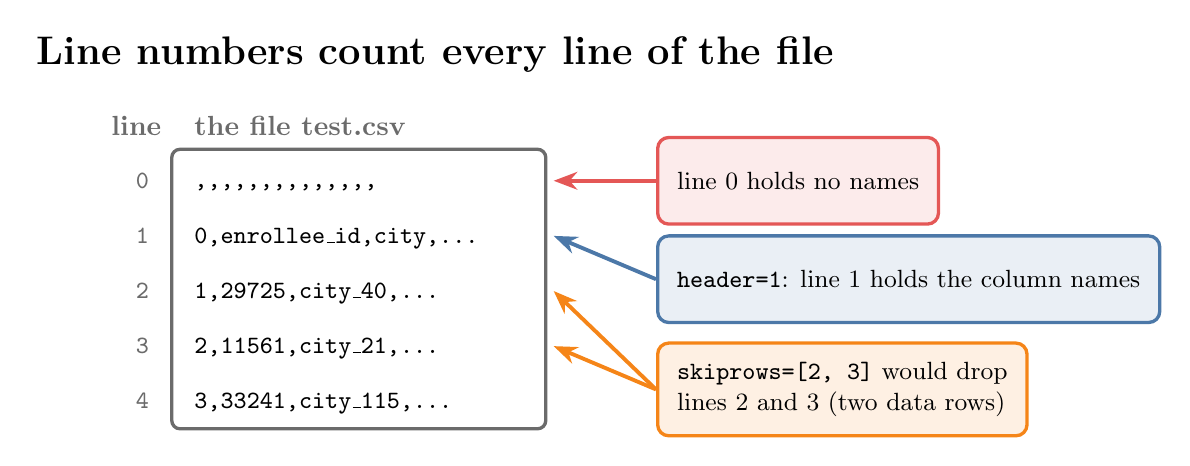
\begin{tikzpicture}[ln/.style={font=\ttfamily\small, text=cgrey, anchor=east},
                    tl/.style={font=\ttfamily\small, anchor=west, text height=1.6ex, text depth=0.4ex}]
  \node[title] at (3.2,3.0) {Line numbers count every line of the file};
  \node[font=\bfseries, text=cgrey] at (-0.6,2.1) {line};
  \node[font=\bfseries, text=cgrey, anchor=west] at (0,2.1) {the file test.csv};
  \node[ln] at (-0.3,1.4) {0}; \node[tl] at (0,1.4) {{,}{,}{,}{,}{,}{,}{,}{,}{,}{,}{,}{,}{,}{,}};
  \node[ln] at (-0.3,0.7) {1}; \node[tl] at (0,0.7) {0,enrollee\_id,city,\dots};
  \node[ln] at (-0.3,0.0) {2}; \node[tl] at (0,0.0) {1,29725,city\_40,\dots};
  \node[ln] at (-0.3,-0.7) {3}; \node[tl] at (0,-0.7) {2,11561,city\_21,\dots};
  \node[ln] at (-0.3,-1.4) {4}; \node[tl] at (0,-1.4) {3,33241,city\_115,\dots};
  \draw[cgrey, rounded corners=3pt] (-0.15,1.8) rectangle (4.6,-1.75);
  % annotations
  \node[box=cred, anchor=west, font=\small] (n0) at (6.0,1.4) {line 0 holds no names};
  \node[box=cblue, anchor=west, font=\small] (n1) at (6.0,0.15) {\texttt{header=1}: line 1 holds the column names};
  \node[box=corange, anchor=west, font=\small, align=left] (n2) at (6.0,-1.25) {\texttt{skiprows=[2, 3]} would drop\\lines 2 and 3 (two data rows)};
  \draw[arrow, draw=cred] (n0.west) -- (4.7,1.4);
  \draw[arrow, draw=cblue] (n1.west) -- (4.7,0.7);
  \draw[arrow, draw=corange] (n2.west) -- (4.7,0.0);
  \draw[arrow, draw=corange] (n2.west) -- (4.7,-0.7);
\end{tikzpicture}
\end{document}
